\documentclass[a4paper]{article}
\usepackage[a4paper, margin=1.5in]{geometry}
\usepackage[utf8]{inputenc}
\usepackage{graphicx} % Required for inserting images
\usepackage[czech]{babel}
\usepackage{amsmath}
\usepackage{amssymb}
\usepackage[T1]{fontenc}
\usepackage{csquotes}
\usepackage{rotating}
\usepackage{hyperref}

\usepackage{lscape}
\usepackage{amsthm}
\usepackage{tikz}
\usetikzlibrary{automata,positioning}
\newtheorem*{statement}{Tvrzení}
\theoremstyle{definition}
\newtheorem*{solution}{Řešení}
\newcommand{\Mod}[1]{
\ \mathrm{mod}\ #1}
%\renewcommand\qedsymbol{\large{$\mathbb{Q.E.D.}$}}
\renewcommand\qedsymbol{\raisebox{-3mm}{\includegraphics[height=6mm]{koteseni.png}}}
\usepackage[parfill]{parskip}
\title{SFC projekt: Demonstrace činnosti GRU sítě}
\author{Bc.\ Vojtěch Vlach (\texttt{xvlach22})}
\newcommand{\rel}[1]{&(x \in #1 \wedge y \in #1)}
\date{2023/24}

\begin{document}

\maketitle

\section{Úvod}
\textbf{Tato dokumentace byla vytvořena v rámci pozdního odevzdání s laskavým dovolením doc. Janouška, kterému tímto děkuji.}

V tomto projektu jsem se rozhodl demonostrovat činnost GRU sítě pomocí jazykové úlohy. Konkrétně rozdělení slov na slabiky. Vytvořil jsem si vlastní dataset a využil jsem implementaci GRU vrstev v  knihovně PyTorch. Pro tuto úlohu již existují řešení, které jsem použil jako referenční baseline a nakonec se mi podařilo baseline výrazně přiblížit, i když jsem ji nepřekonal.

\section{Popis úlohy}

Pro tento projekt jsem si zvolil úlohu rozdělení slova na slabiky. Omezil jsem se pouze na česká slova, kde mohu posoudit správnost intuitivně. Přesněji se tedy jedná o problém, kde na vstupu je české slovo a na výstupu by mělo být slovo rozdělené na slabiky. Nenalezl jsem mnoho literatury, která by se tímto problémem zabývala, předpokládám, že je to úloha moc jednoduchá na to, aby se na tom dal zveřejňovat seriózní článek. Výjimku tvoří např. Hyphenation using Deep Neural Network\footnote{\href{https://negedng.github.io/files/2018-Hyphenation.pdf}{Gergely et al. Hyphenation using Deep Neural Network}}.

\subsection{Získání datasetu}

Pro výrobu datasetu jsem využil fonetický korpus Češtiny\footnote{\href{https://ujc.avcr.cz/phword}{The Phonological Corpus of Czech}}, který se zabývá kromě fonetické výslovnosti češtiny také četnostmi výskytu fonémů, slov a slabik. Konkrétně jsem využil následující sadu: \href{http://www.ujc.cas.cz/phword/ssc_29-06-16.zip}{Lexemes from Slovník spisovné češtiny, 4th edition, 2005}, která obsahuje právě fonetický přepis a jeho rozdělení na slabiky, které jsem využil. Slova v datasetu byly ve formátu, které jsou naznačeny ve sloupcích \texttt{Původní slovo}, \texttt{Fonetický přepis} a \texttt{Fonetické slabiky} viz tabulka \ref{table:dataset}.

Z těchto sloupců jsem jednoduchým algoritmem získal přepis na slabiky. Program procházel sloupce \texttt{Původní slovo} a \texttt{Fonetické slabiky} současně, nahrazoval fonetické výrazy původními písmeny a zanechal u nich informaci o slabikách. Více viz Python Notebook \texttt{python-scripts/Dataset\_creating.ipynb}.
Dále jsem získaná slova rozdělil na datasety v následujících variantách (první číslo je počet slov určených k trénování a druhé číslo je počet slov k validaci): 1000-250, 10000-2500, 30000-8000. Tyto sady jsou k dostání ve složkách \texttt{dataset/ssc\_29-06-16/set\_\dots{}}.

Pro zhodnocení jsem ručně vytvořil sadu 100 dlouhých slov, která je k dostání v souboru \texttt{dataset/long\_words\_test.txt}.

\section{Formulování úlohy modelu}

V rámci projektu jsem experimentoval se dvěma způsoby. První způsob je regresního typu a využívá Mean-Square Error jako chybovou funkci. Druhý způsob (vytvořen v rámci pozdního odevzdání) funguje na principu binární klasifikace a Cross-entropy loss jako chybové funkce.
Oba přístupy zpracovávají vstupní slovo jako posloupnost písmen a liší se ve formulaci ground-truths. Délka vstupu a výstupu je vždy stejná a oba modely nahradí poslední písmeno slabiky příslušnou třídou. Doplnění oddělovače do výsledného slova (např. \texttt{-}) zajistí jednoduchý algoritmus. Tento způsob jsem zvolil proto, aby se nezpožďovaly výstupní písmena od těch vstupních. 

\subsection{Regresní přístup}

Ground-truths u tohoto přístupu tvoří přímo písmena (jejich index v abecedě), ke kterému by se měl model postupně blížit. Token pro konec slabiky je zde speciální znak (\texttt{@}). 
Příklad tohoto zpracování je v sloupci \texttt{Ground truth multi}, viz Tabulka \ref{table:dataset}

\subsection{Binární klasifikace}

Ground-truth zde tvoří pouze třídy 2 třídy, kde 1 znamená poslední písmeno slabiky, 0 znamená opak.
Příklad tohoto zpracování je v sloupci \texttt{Ground truth bin}, viz Tabulka \ref{table:dataset}


\begin{table}[]
\centering
\caption{Tabulka 1: Proces získání datové sady.}
\begin{tabular}{|l|l|l|}
\hline
\textbf{Původní slovo}     & \textbf{Fonetický přepis}    & \textbf{Fonetické slabiky} \\ \hline
adresa                     & adresa                       & a.dre.sa                   \\ \hline
antimilitaristický         & antimilitariStiTSkí          & an.ti.mi.li.ta.riS.tiTS.kí \\ \hline
antikvariát                & antikvarijáT                 & an.ti.kva.ri.jáT           \\ \hline
popřípadě                  & popřípadě                    & po.pří.pa.ďe               \\ \hline
\textbf{Přepis na slabiky} & \textbf{Ground truth bin}    & \textbf{Ground truth multi}      \\ \hline
a-dre-sa                   & 100100                       & @dr@sa                     \\ \hline
an-ti-mi-li-ta-ris-tic-ký  & 010101010100100100           & a@t@m@l@t@ri@ti@ky         \\ \hline
an-ti-kva-ri-át            & 01010010110                  & a@t@kv@r@@t                \\ \hline
po-pří-pa-dě               & 010010100                    & p@pr@p@de                  \\ \hline
\end{tabular}
\label{table:dataset}
\end{table}

\subsection{Baseline}

Baseline pro zhodnocení jsem zvolil knihovnu pyphen pro python, která podporuje češtinu a funguje na algoritmu, který se používá jako standard pro dělení slov v programu \Latex{} TODO check LATEX. a dalších textových programech.

\section{Implementace}
Všechny implementované skripty popsané v této kapitole jsou k nalezení ve složce \texttt{src}. Jsou to:

TODO: add bullet list
 - train.py: hlavní funkce s trénovacícm cyklem
 - net_definitions.py: definice obou modelů
 - gui.py: jednoduchá grafická aplikace
 - inference.py: manuální testování
 - test.py: automatické testování
 - pomocné skripty: helpers.py, charset.py, dataset.py

Pro svoji implementaci jsem se inspiroval článkem Gated Recurrent Unit (GRU) With PyTorch\footnote{\href{https://blog.floydhub.com/gru-with-pytorch/}{Loye Gabriel, 2019: Gated Recurrent Unit (GRU) With PyTorch}}, který ukazuje možnost využití pro predikci časové řady. Jeho řešení jsem si upravil, aby vyhovovalo mojí úloze.

\paragraph{Původní GRU s regresním přístupem.}
Původní implementací modelu je třída \texttt{GRUNet} v souboru \texttt{src/net\_definitions.py}, která definuje jednoduchou rekurentní síť s plně propojenou vrstvou na výstupu. Struktura sítě je definována jako GRU vrstva (+ ReLU aktivace) a plně propojená vrstva pro agregování vektoru skrytého stavu na formát výstupu. Vizualice je na Obrázku \ref{png:gru_old_adresa}.

\begin{figure*}[t!]
  \centering
  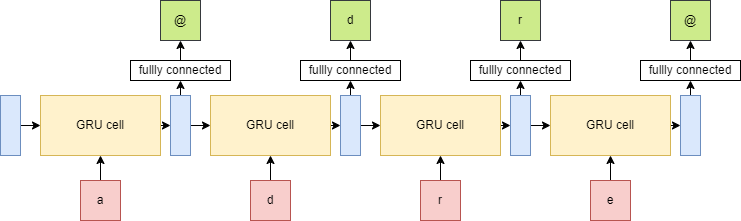
\includegraphics[width=4.5in]{gru_diagram_adresa.png}\\[1pt]  % width=\linewidth,hineight=1.7in
  \caption{Znázornění činnosti sítě pro začátek slova \texttt{adresa}.\\Červená: vstup, žlutá: GRU buňka, bílá: plně propojená vrstva, modrá: vektor skrytého stavu, zelená: výstup sítě.}
  \label{png:gru_old_adresa}
\end{figure*}

\paragraph{GRU s binární klasifikací}
V druhém případě jsem definoval nový model, který využívá embedding vrstvu kódující vstupní znaky do vektorů. Dále obsahuje GRU vrstvu následovanou dekodérem ve formě plně propojené vrstvy, který výsledný skrytý vektor opět zmenší na pouze jedno číslo. Výstup je aktivován pomocí sigmoidy, která jakýkoliv vstup zmenší do intervalu od 0 do 1. Na tomto výstupu se pak dá jednoduše provést binární klasifikace pro každé písmeno zvlášť.

\paragraph{Funkce train.}
Dále jsem naimplementoval funkci train, která spouští trénování pomocí zadaných paramterů. \textit{Umožňuje procházet dataset rozdělený na dávky a pro každý spočítá chybu a provede optimalizační krok.} Jako chybovou funkci využívá \texttt{Mean\ Square\ Error} resp. \texttt{Binární Cross-entropy} a k optimalizačním krokům využívá optimalizátor \texttt{Adam}, Dále umožňuje nahrát dříve uložený model a pokračovat v trénování. V průběhu shromažďuje statistiky o chybách a jednou za \texttt{save\_step} epoch uloží aktuální stav modelu a grafy znázorňující průběh chyby na trénovací i validační sadě.

\paragraph{Další části implementace.}
Další části důležité pro běh trénování jsou tyto soubory \texttt{charset.py} (obsahující definici kódování slov ze \texttt{stringu} na \texttt{float tensor} popř. \texttt{int tensor} podle zvoleného přístupu), \texttt{helpers.py} (obsahující podpůrné funkce pro trénování: počítání levenshteinovy vzdálenosti, ukládání a nahrávání modelu a vytváření grafů), \texttt{dataset.py} (obsahující stejnojmennou třídu, která nahrává soubor a zpracovává ho na vstupy sítě a ground-truths a poskytuje možnost iterování přes batche),


\section{Spuštění + ovládání}

Pro spuštění by měl stačit python3.8+. První krok je nainstalování všech potřebných knihoven pomocí skriptu \texttt{install.sh}. Dále stačí spouštět skripty pomocí příkazové řádky.

Pro spuštění trénování podle nastavených parametrů přímo v kódu je následující příkaz: \\
\texttt{python3 src/train.py}

Pro manuální testování modelu je připraven soubor \texttt{src/inference.py}, který nabízí jednoduchý CLI interface k modelu. Je spustitelný pomocí příkazu: \\
\texttt{python3 src/inference.py}

pozn. pro úpravy a spouštění python notebooku \texttt{Dataset\_creating.py} je navíc potřeba prostředí pro Jupyter Notebook.

\section{Výsledky}

\subsection{Regresní přístup}
\label{subsec:regresion}

Konkrétně jsem zkoušel model s následujícími hyperparametry. Velikost skrytého vektoru: 8, výstupy GRU vrstvy byly zpracovány pouze ReLU a poté plně propojenou vrstvou. viz \ref{png:gru_old_adresa}.
V této konfiguraci se nepodařilo natrénovat model, který by měl uspokojivé výsledky. Model se v rámci experimentu nedokázal naučit ani základní opakování písmen a na výstupu dává chybná písmena téměř ve všech testovaných případech. Chyba trénování se postupně zmenšovala, ale později se ustálila. Model tedy už pojal veškeré informace, které mohl a neměl další prostor na učení.
V tomto stavu se tedy lze bavit pouze o demonstraci postupného zmenšování chyby, ale nikoliv praktického použití. Příklady viz Tabulka \ref{table:vystupy_old_gru}

\begin{table}[]
\caption{Tabulka 2: Příklad výstupů nedotrénovaného modelu.}
\begin{tabular}{|l|l|l|}
\hline
\textbf{Vstup} & \textbf{Ground-truth}               & \textbf{Výstup}                     \\ \hline
vyhotovovat    & v@h@t@v@vat\_\_\_\_\_\_\_\_\_       & uxquvvuuvdt\_\_\_\_\_\_\_\_\_       \\ \hline
cecko          & ce@ko\_\_\_\_\_\_\_\_\_\_\_\_\_\_\_ & epmnu\_\_\_\_\_\_\_\_\_\_\_\_\_\_\_ \\ \hline
vynalez        & v@n@lez\_\_\_\_\_\_\_\_\_\_\_\_\_   & uxrtnpw\_\_\_\_\_\_\_\_\_\_\_\_\_   \\ \hline
\end{tabular}
\label{table:vystupy_old_gru}
\end{table}

\subsection{Binární klasifikace}

V tomto případě jsem použil komplexnější strukturu sítě, která se ukázala být velice efektivní na danou úlohu. Nejvíc osvědčené hyperparametry byly následující. Velikost skrytého vektoru: 256, GRU vrstev: 2, obousměrný GRU průchod.

Pomocí většího skrytého vektoru získal model možnost uchovat si víc informací. Díky zjednodušení úlohy na binární klasifikaci se výrazně zjednodušilo trénování a hned ve výchozím stavu model umí alespoň zopakovat vstup (Regresnímu přístupu se ani toto nepodařilo). Dále pomocí obousměrného průchodu získal model možnost agregovat informaci nejen z předchozích vstupů, ale i těch následujících. Příklad trénování lze vidět na obrázku \ref{png:graf_trenovani_new_gru}. Lze z něj vidět, že trénovací chyba postupně osciluje na ustálených malých hodnotách, při většině trénování byla úspěšnost na trénovací sadě 100 \%. úspěšnost na validační sadě se už ale zdá být ustálená.

\begin{figure*}[t!]
  \centering
  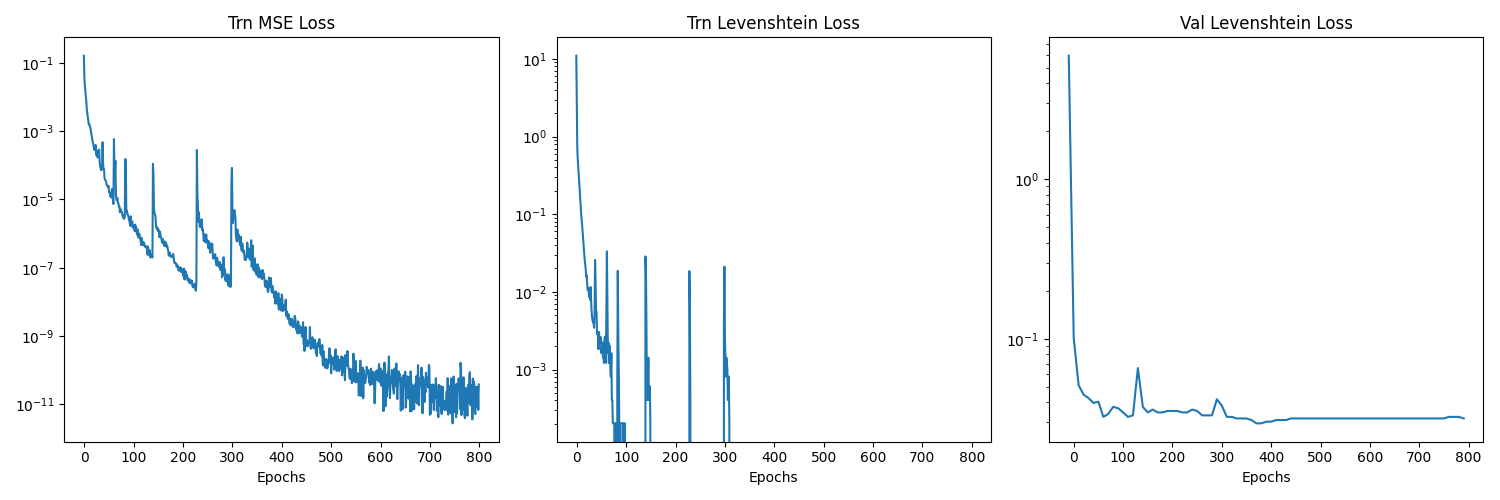
\includegraphics[width=4.5in]{docs/torch_gru_256hid_2layers_bidirectional_yesbias_250batch_800epochs.png}\\[1pt]  % width=\linewidth,hineight=1.7in
  \caption{Průběh trénování Binární klasifikace. Zleva: Průběh chyby binární cross entropie (popisek v grafu MSE je chyba), průběh Levenshteinovy vzdálenosti na trénovací sadě (v místech, kde mizí čára, byla chyba nulová), průběh Levenshteinovy vzdálenosti na validační sadě v setinách procent}
  \label{png:graf_trenovani_new_gru}
\end{figure*}

\subsection{Zhodnocení}
\label{subsec:zhodnoceni}

Pro otestování funkčnosti modelů jsem použil testovací sadu neviděných slov a chybu vyhodnotil pomocí levenshteinovy vzdálenosti, která značí podíl elementárních úprav, které je potřeba k opravení výstupu na ground-truth vůči celkové délce grount-truth.

GRU s regresním přístupem dosáhlo 83.41 \%, GRU s binární klasifikací dosáhlo 7.53 \% a baseline algoritmus dosáhl 1.5 \%. 

Lze tedy vidět, že žádný z modelů pro danou testovací sadu nepřekonal baseline algoritmus.
Důvod neúspěchu v tolika případech může být např. nedostatečně rozmanitá trénovací sada. Je možné, že díky nedokonalému procesu vytváření, v sadě chybí zástupci některých případů.

TODO table?
GRU old Levenshtein loss:  83.41 %
GRU new Levenshtein loss:  7.53 %
Baseline Levenshtein loss: 1.50 %


\section{Závěr}
V rámci tohoto projektu jsem se věnoval vývoji modelu pro dělení českých slov na slabiky za využití GRU vrstev. Otestoval jsem dva hlavní přístupy k úloze: regresní přístup s chybovou funkcí \texttt{Mean\_square\_error} a binární klasifikaci s chybovou funkcí \texttt{Binární cross-entropy}. První přístup se nepodařilo přimět k uspokojivým výsledkům. Možné důvody jsou popsaná v sekci \ref{subsec:regresion}. Druhý přístup dosáhl své maximální kapacity a pro trénovací i validační sady. Po zhodnocení pomocí neviděných dat ale neporazil baseline algoritmus a další krok by tedy mohl být např. větší prozkoumání případů chybné klasifikace a doplnění případných nedostatečných příkladů do trénovací a validační sady.

Díky tomuto projektu jsem se naučil používat knihovnu pytorch pro definici vlastních modelů a osvojil si i trénovací cyklus používaný obecně pro vývoj v oboru strojového učení. Projekt dále slouží jako demonstrace činosti GRU vrstvy v několika modifikacích.

\end{document}
